\section*{Direction 3. Can one predator--prey equation predict outcomes in other biological systems?}

\subsection*{Abstract}
We tested the course equation on five experimental settings in which one population affects another. On a glioma cell line, the equation gave lower mean prediction error than CARRGO, a model for chimeric antigen receptor (CAR) T-cell therapy. A model that tracks stages of infection was more accurate in 11 of 12 four-hour bacteriophage tests. A separate leukemia dataset measured both interacting populations. Fitting the equation to both populations recovered all twelve early T-cell increases, but more than doubled the mean error for the target cells. A mathematical comparison explains how an accurate target forecast can depend only weakly on the modeled interaction.

\subsection*{Results}
\textbf{What transferred between systems.}
We kept the original two equations and fitted their seven positive coefficients using the training conditions in each assay. Writing $x$ for the target and $y$ for the consumer gives
\[
 \dot x=xg(x)-F(x,y),\qquad \dot y=eF(x,y)-dy,\qquad
 g(x)=r(1-x/K)(1+\alpha x),\quad F(x,y)=\frac{mxy}{\beta+y}.
\]
Here $g$ is the course model's per-capita prey growth law. Per-capita growth initially increases with density when $\alpha K>1$. The term $F$ removes targets, and the same flux contributes $eF$ to consumer growth. In the cell assays, the target is a tumor cell population and the consumer represents T cells. In the phage assays, $x$ represents bacteria and $y$ represents phage.

\textbf{What counted as a successful prediction.}
Each test held out a whole dose, input level, or population ratio. We scored errors on the measurement scale of that assay. Cell Index (CI) measures electrical impedance, optical density (OD) measures a culture's effect on transmitted light, and the leukemia assay reports marker-positive cell counts. Root-mean-square error (RMSE) is the square root of the mean of the squared differences between predictions and observations. Smaller values indicate closer predictions. Means across conditions give each held condition equal weight.

\textbf{Which target forecasts relied on the consumer?}
For each ecological fit to the cell-line data, we kept all coefficients and the starting target level fixed and set the starting consumer to zero. In the six primary PBT138 tests, this changed the predicted target by a maximum of 2.20--2.54 CI on the held time grids. In five of six HT1080 tests the maximum change was below 0.000052 CI. The sixth reached 0.07934 CI. The same equation therefore assigned very different roles to the interacting population.

\textbf{Which forecast was tested?}
The main comparisons transferred the equation and fitted its coefficients to training conditions in each assay. Separate tests froze those coefficients before forecasting a different cell line or acquisition. The leukemia study added a second measured population, allowing the target forecast and the consumer forecast to be scored separately.

\clearpage
\subsection*{Figures and tables}
\subsubsection*{Held target measurements across assays}
\begin{center}
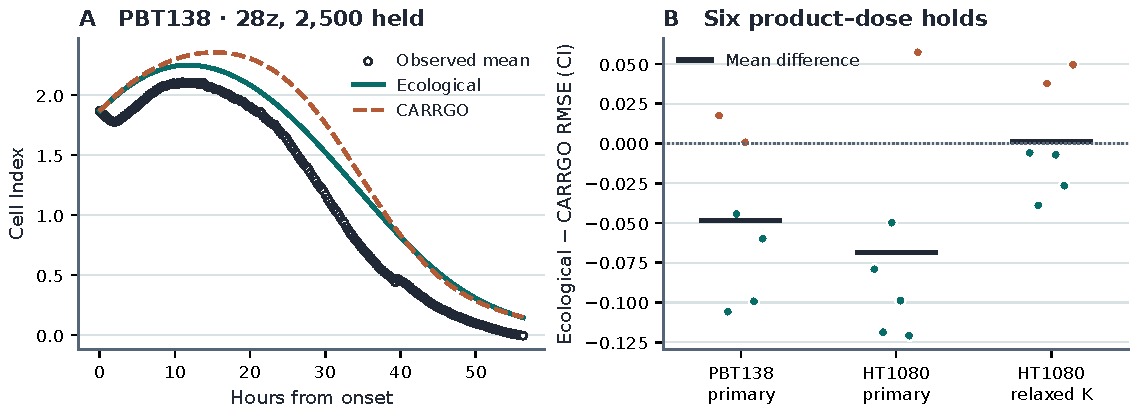
\includegraphics[width=.93\linewidth]{d3/figures/cart_held.pdf}
\captionof{figure}{Cell Index after a held dose. At left, points and lines refer to one held PBT138 condition. At right, each point is an ecological-minus-CARRGO RMSE difference for one of six conditions. A negative value favors the ecological equation.}
\end{center}
In PBT138, the ecological equation won four of six held conditions, with mean errors of 0.288 CI for ecology and 0.336 CI for CARRGO. For HT1080, the untreated controls reached 10.118 CI, above the original capacity ceiling of 10. Raising only that ceiling changed the mean errors from 0.3052 and 0.3736 CI to 0.1993 and 0.1978 CI, respectively. Freezing the coefficients across cell lines gave ecological and CARRGO errors of 0.587 and 0.519 CI from PBT138 to HT1080, and 1.700 and 1.015 CI in reverse, over 24 hours.

\begin{center}
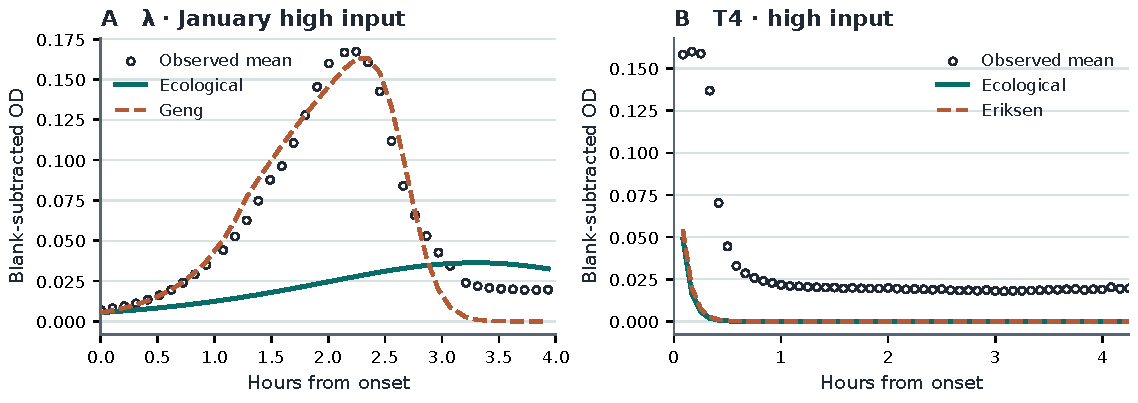
\includegraphics[width=.93\linewidth]{d3/figures/phage_held.pdf}
\captionof{figure}{Optical density at a held high input in two independent assays. Points are mean observations and curves are model predictions. The January $\lambda$ assay used Geng's infection-stage model as the comparator. The T4 assay used Eriksen's resource model.}
\end{center}
Geng's model had lower four-hour error in 11 of 12 held inputs across four $\lambda$ acquisitions. On independent T4 data, ecology won two of three inputs over 4.25 hours and one of three over the first hour. A separate transfer experiment froze January's $\lambda$ parameters and scored 18 positive conditions on three later dates. Ecology then had lower mean four-hour error (0.0628 vs.\ 0.0747 OD), although it won only eight individual comparisons. The average and the number of wins give different information about the size of the errors.

\clearpage
\subsubsection*{Predicting both populations with one parameter vector}
The LT6 leukemia assay recorded CD33-positive targets and total CD3-positive T cells. Each of two target genotypes, wild type (WT) and TP53 knockout (KO), had six treated ratios. For each held ratio, we fitted on the other five ratios of the same genotype and included target values from the untransduced controls. One vector then predicted both markers at days 6, 10, and 16 from the held condition's measured day-3 counts. The twelve comparisons describe one acquisition and share training data.

\begin{center}
\captionof{table}{Primary LT6 results. The two error columns give mean RMSE across the twelve held conditions in dilution-corrected cell counts. The last column counts correct predictions of the observed CD3 increase from day 3 to day 6.}
\small
\begin{tabular}{@{}lrrr@{}}\toprule
Model and fitting rule & CD33 RMSE & CD3 RMSE & Early rises \\\midrule
Ecology, target only & 81,634 & 6,099 & 0/12 \\
Ecology, 5\% target-loss band & 83,611 & 5,025 & 10/12 \\
Ecology, equal-weight joint fit & 197,580 & 4,990 & 12/12 \\
CARRGO, equal-weight joint fit & 177,505 & 5,095 & 11/12 \\
Shah Beddington--DeAngelis, joint fit & 134,300 & 4,594 & 12/12 \\
Growth model and constant CD3 & 81,648 & 5,019 & 0/12 \\
Growth model and day-specific CD3 & 81,648 & 2,039 & 12/12 \\\bottomrule
\end{tabular}
\end{center}
Equal-weight training used the sum of the two normalized marker losses. The 5\% rule selected for lower CD3 training loss among candidates within 5\% of the lowest CD33 training loss found. The day-specific CD3 reference multiplied the held starting count by the median change factor among training ratios at each forecast day. It gave a lower CD3 RMSE than the joint ecological fit in all twelve conditions.

\begin{center}
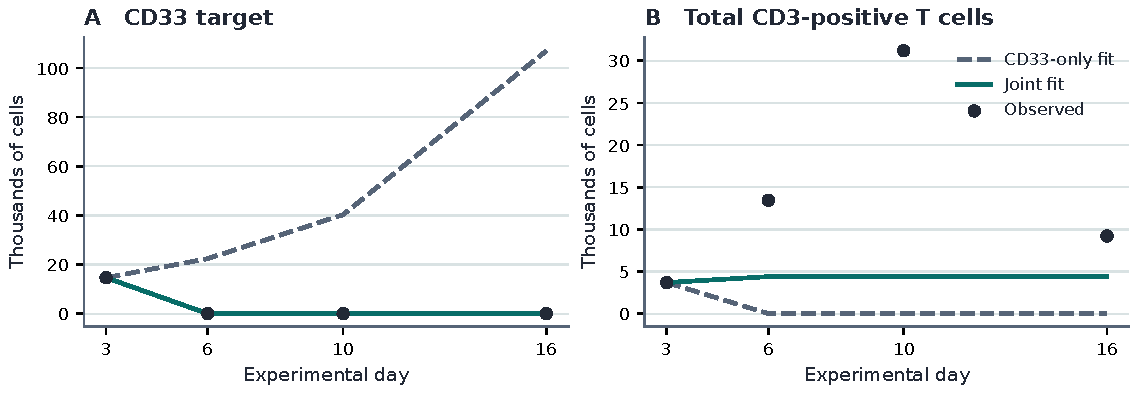
\includegraphics[width=.94\linewidth]{d3/figures/aml_case.pdf}
\captionof{figure}{Held wild-type 1:16 condition. Both fits used the same day-3 measurements. The joint fit predicted the rapid loss of CD33-positive targets closely (RMSE 21.7 counts). It predicted about 4,393 CD3-positive cells on day 10, when 31,180 were observed.}
\end{center}
At fixed joint coefficients, retaining the consumer improved CD33 error relative to setting its initial value to zero in three of twelve conditions. Across all twelve, mean CD33 RMSE was 197,580 with the consumer and 131,587 without it. Total CD3 includes cells whose functional activity was unmeasured.

\clearpage
\subsection*{Mathematical proof}
\textbf{How much can the consumer change a target forecast?}
Take positive coefficients and initial values $x_0,y_0>0$. On $[0,T]$, compare the positive interacting solution $(x,y)$ with the solution $(X,0)$ from $(x_0,0)$ using the same coefficients. Set
\[
 M=\max(K,x_0),\quad A=\alpha K,\quad
 \gamma=d-\frac{emM}{\beta},\quad L=\frac{r\max(A-1,0)^2}{8A}.
\]
If $\gamma>0$, then for $0\le t\le T$,
\[
 0\le X(t)-x(t)\le M(1-e^{-Z_T}),\qquad
 Z_T=e^{LT}\frac{m}{\gamma}\log(1+y_0/\beta).
\]

\textit{Proof.}
Write $h(y)=my/(\beta+y)$. On a regular trajectory the consumer satisfies
$\dot y=y\{emx/(\beta+y)-d\}$. Integrating this linear equation in $y$ along the trajectory shows that a zero initial consumer remains zero. Its associated target therefore solves $\dot X=Xg(X)$. A positive initial state remains positive on the solution interval by the same factorization for each population. At $M$ the two target derivatives are nonpositive. Since $\dot x\le xg(x)$, scalar comparison gives $0<x\le X\le M$.

It follows that $\dot y/y\le-\gamma$ and $y(t)\le y_0e^{-\gamma t}$. Monotonicity of $h$ gives
\[
 \int_0^t h(y(s))\,ds
 \le \int_0^\infty \frac{my_0e^{-\gamma s}}{\beta+y_0e^{-\gamma s}}\,ds
 =\frac{m}{\gamma}\log(1+y_0/\beta).
\]
The derivative of $g(x)$ with respect to $\log x$ is the quadratic
$xg'(x)=r[(\alpha-1/K)x-2\alpha x^2/K]$. Its supremum for $x>0$ is $L$. The vertex gives $r(A-1)^2/(8A)$ for $A>1$, and the supremum is zero as $x\downarrow0$ for $A\le1$. Hence
$z=\log(X/x)\ge0$ satisfies $\dot z=g(X)-g(x)+h(y)\le Lz+h(y)$.
Integrating from $z(0)=0$ gives $z(t)\le Z_T$.
Finally $X-x=X(1-e^{-z})\le M(1-e^{-Z_T})$.

\textbf{Why this protects the target-error rankings.}
On a common grid of $n\ge1$ observations $o$, write $E(u)=\|u-o\|_2/\sqrt n$.
The reverse triangle inequality gives
$|E(u)-E(v)|\le\|u-v\|_2/\sqrt n\le\max_i|u_i-v_i|$.
Thus a strict error gap to a comparator survives any smaller uniform change in the forecast. On the 13-day LT6 window, the largest target-only displacement bounds were 143.16 counts under primary bounds and 37.20 under expanded bounds. The smallest comparator gaps were 898.93 and 1,109.93 counts, respectively. All $12\times2\times3=72$ rankings therefore survived removal of the consumer. The three comparators were CARRGO, Shah Beddington--DeAngelis, and the fixed-dose model. For primary joint ecological fits, $\gamma>0$ failed in all twelve conditions. Their fixed-coefficient comparisons used direct numerical integration.

\begin{center}
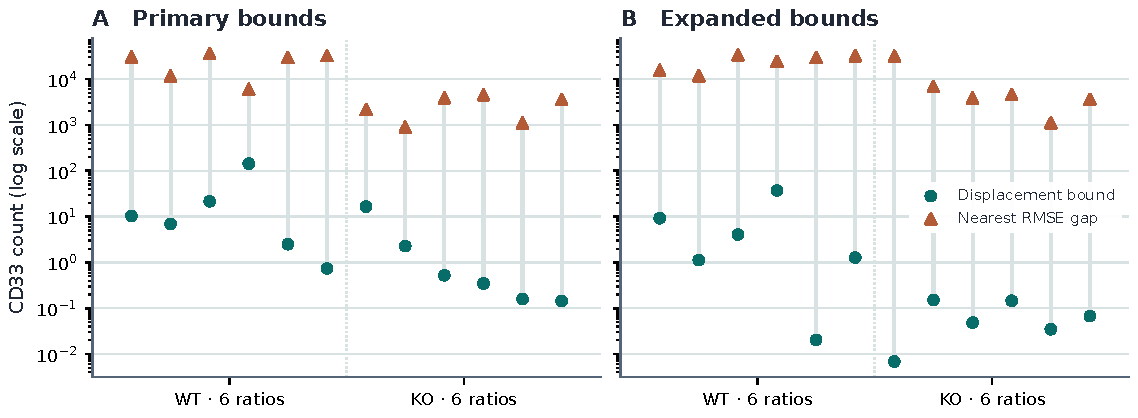
\includegraphics[width=.84\linewidth]{d3/figures/ablation_certificate.pdf}
\captionof{figure}{Each circle gives the target displacement bound for one of the twelve held LT6 ratios. The triangle above it gives the smallest RMSE gap to any comparator. The two panels use the same condition order and report dilution-corrected CD33 counts on a logarithmic scale.}
\end{center}

\clearpage
\subsection*{Python code}
This example scores the equal-weight joint forecast for the held wild-type 1:16 condition in Figure~3.3. Inputs are dilution-corrected counts on days 3, 6, 10, and 16. Forecast values are rounded for display. Day 3 initializes the forecast, so the error uses only the last three dates.

\begin{lstlisting}[language=Python,basicstyle=\ttfamily\footnotesize]
from math import sqrt
from statistics import mean

observed_cd33 = (14656.2, 37.6, 0.0, 0.0)
forecast_cd33 = (14656.2, 0.0, 0.0, 0.0)
observed_cd3 = (3687.6, 13463.2, 31179.5, 9212.1)
forecast_cd3 = (3687.6, 4393.245, 4393.228, 4393.201)

def rmse(observed, forecast):
    pairs = zip(observed[1:], forecast[1:])
    return sqrt(mean((o - p)**2 for o, p in pairs))

print(round(rmse(observed_cd33, forecast_cd33), 1))
print(round(rmse(observed_cd3, forecast_cd3), 1))
print(forecast_cd3[1] > forecast_cd3[0] + 1e-7)
\end{lstlisting}
The outputs are 21.7 CD33 counts, 16,562.9 CD3 counts, and \texttt{True} for the early rise. The averages in Table~3.1 give equal weight to each of the twelve held conditions.

\subsection*{Lean verification results}
Lean 4.19.0 with Mathlib v4.19.0 checked 22 public declarations. For regular solutions on a finite interval, it verified that zero initial consumer density stays zero and that the target then follows its scalar growth equation with the original parameters and initial target. It also verified the conditional upper bound on consumer density, the RMSE inequality, and the resulting sufficient condition for preserving an error ranking.

Two proofs verify that the twelve genotype--ratio pairs are distinct and that the observed CD3 count rose from day 3 to day 6 in each. Both proofs use no axioms. Python matched the 24 counts to the published LT6 observations. The preceding page derives the full target displacement bound and applies it to 72 forecast comparisons.
